%% ****** Start of file apstemplate.tex ****** %
%%
%%
%%   This file is part of the APS files in the REVTeX 4.2 distribution.
%%   Version 4.2a of REVTeX, January, 2015
%%
%%
%%   Copyright (c) 2015 The American Physical Society.
%%
%%   See the REVTeX 4 README file for restrictions and more information.
%%
%
% This is a template for producing manuscripts for use with REVTEX 4.2
% Copy this file to another name and then work on that file.
% That way, you always have this original template file to use.
%
% Group addresses by affiliation; use superscriptaddress for long
% author lists, or if there are many overlapping affiliations.
% For Phys. Rev. appearance, change preprint to twocolumn.
% Choose pra, prb, prc, prd, pre, prl, prstab, prstper, or rmp for journal
%  Add 'draft' option to mark overfull boxes with black boxes
%  Add 'showkeys' option to make keywords appear
\documentclass[aps,prl,preprint,groupedaddress]{revtex4-1}
%\documentclass[aps,prl,preprint,superscriptaddress]{revtex4-2}
%\documentclass[aps,prl,reprint,groupedaddress]{revtex4-2}
\usepackage{amsmath}
\usepackage{subfig}
\usepackage{rotating}
\usepackage{graphics}
\usepackage{graphicx}
\usepackage{subfig}
% You should use BibTeX and apsrev.bst for references
% Choosing a journal automatically selects the correct APS
% BibTeX style file (bst file), so only uncomment the line
% below if necessary.
%\bibliographystyle{apsrev4-2}

\begin{document}

% Use the \preprint command to place your local institutional report
% number in the upper righthand corner of the title page in preprint mode.
% Multiple \preprint commands are allowed.
% Use the 'preprintnumbers' class option to override journal defaults
% to display numbers if necessary
%\preprint{}

%Title of paper
\title{Voltage pulse unveils a far away perturbation}

% repeat the \author .. \affiliation  etc. as needed
% \email, \thanks, \homepage, \altaffiliation all apply to the current
% author. Explanatory text should go in the []'s, actual e-mail
% address or url should go in the {}'s for \email and \homepage.
% Please use the appropriate macro foreach each type of information

% \affiliation command applies to all authors since the last
% \affiliation command. The \affiliation command should follow the
% other information
% \affiliation can be followed by \email, \homepage, \thanks as well.
\author{Auteurs}
%\email[]{Your e-mail address}
%\homepage[]{Your web page}
%\thanks{}
%\altaffiliation{}
\affiliation{CEA, N\'{e}el}

%Collaboration name if desired (requires use of superscriptaddress
%option in \documentclass). \noaffiliation is required (may also be
%used with the \author command).
%\collaboration can be followed by \email, \homepage, \thanks as well.
%\collaboration{}
%\noaffiliation

\date{\today}

\begin{abstract}
% insert abstract here
Here we present the unveilling of dynamical interferences in a Fermi liquid by a voltage pulse propagating through a quantum wire. Time-dependent simulations were performed with the opensource Python package Kwant and its extension Tkwant.
\end{abstract}

% insert suggested keywords - APS authors don't need to do this
%\keywords{}

%\maketitle must follow title, authors, abstract, and keywords
\maketitle

% body of paper here - Use proper section commands
% References should be done using the \cite, \ref, and \label commands
\section{Introduction}
% Put \label in argument of \section for cross-referencing
%\section{\label{}}


\section{Model}
%We consider a N sites one dimensional wire connected to two semi-infinite leads. We model the system by the following tight-binding Hamiltonian:
\begin{equation}
\textbf{H} = -\gamma \sum_{i}c^{\dagger}_i c_{i+1} + \sum_{i} w(t)\theta(-i) c^{\dagger}_i c_{i} + \sum_{i} V_{QPC}(i) c^{\dagger}_i c_{i}
\end{equation}
The scattering region will be indexed by $i \in [\![1,N]\!]$, whereas left (right) lead sites are indexed with $i \leq 0$
 ($i \geq N+1$). The hopping  The voltage pulse is modeled by the second term, with $\theta(x)$ being the Heaviside function and $w(t)$:
 \begin{equation}
 	w(t) = V_P e^{-2(\frac{t-t_0}{\tau})^2}
 \end{equation}
 $V_P$ being the amplitude, $\tau$ the width and $t_0$ the starting time of the perturbation. We introduced a Quantum Point Contact (QPC) which consists in a filtering potential barrier:
 \begin{equation}
V_{QPC}(i) = V_0 e^{-(\frac{i - i_0}{\xi})^2}
 \end{equation}
 $V_0$ being the amplitude, $\xi$ the width and $x_0$ the position of the QPC.
 The time-dependent peturbation can be absorbed by the gauge transforming leading to a redefinition of the hopping parameter the left lead where the pulse is applied and the scattering region:
 \begin{equation}
\gamma \rightarrow \gamma e^{-i\phi(t)}
 \end{equation}
 with:
 \begin{equation}
 	\phi(t) = \frac{e}{\hbar}\int_{-\infty}^{t} w(u)du
 \end{equation}
 
\begin{figure}[h]
	\centering
	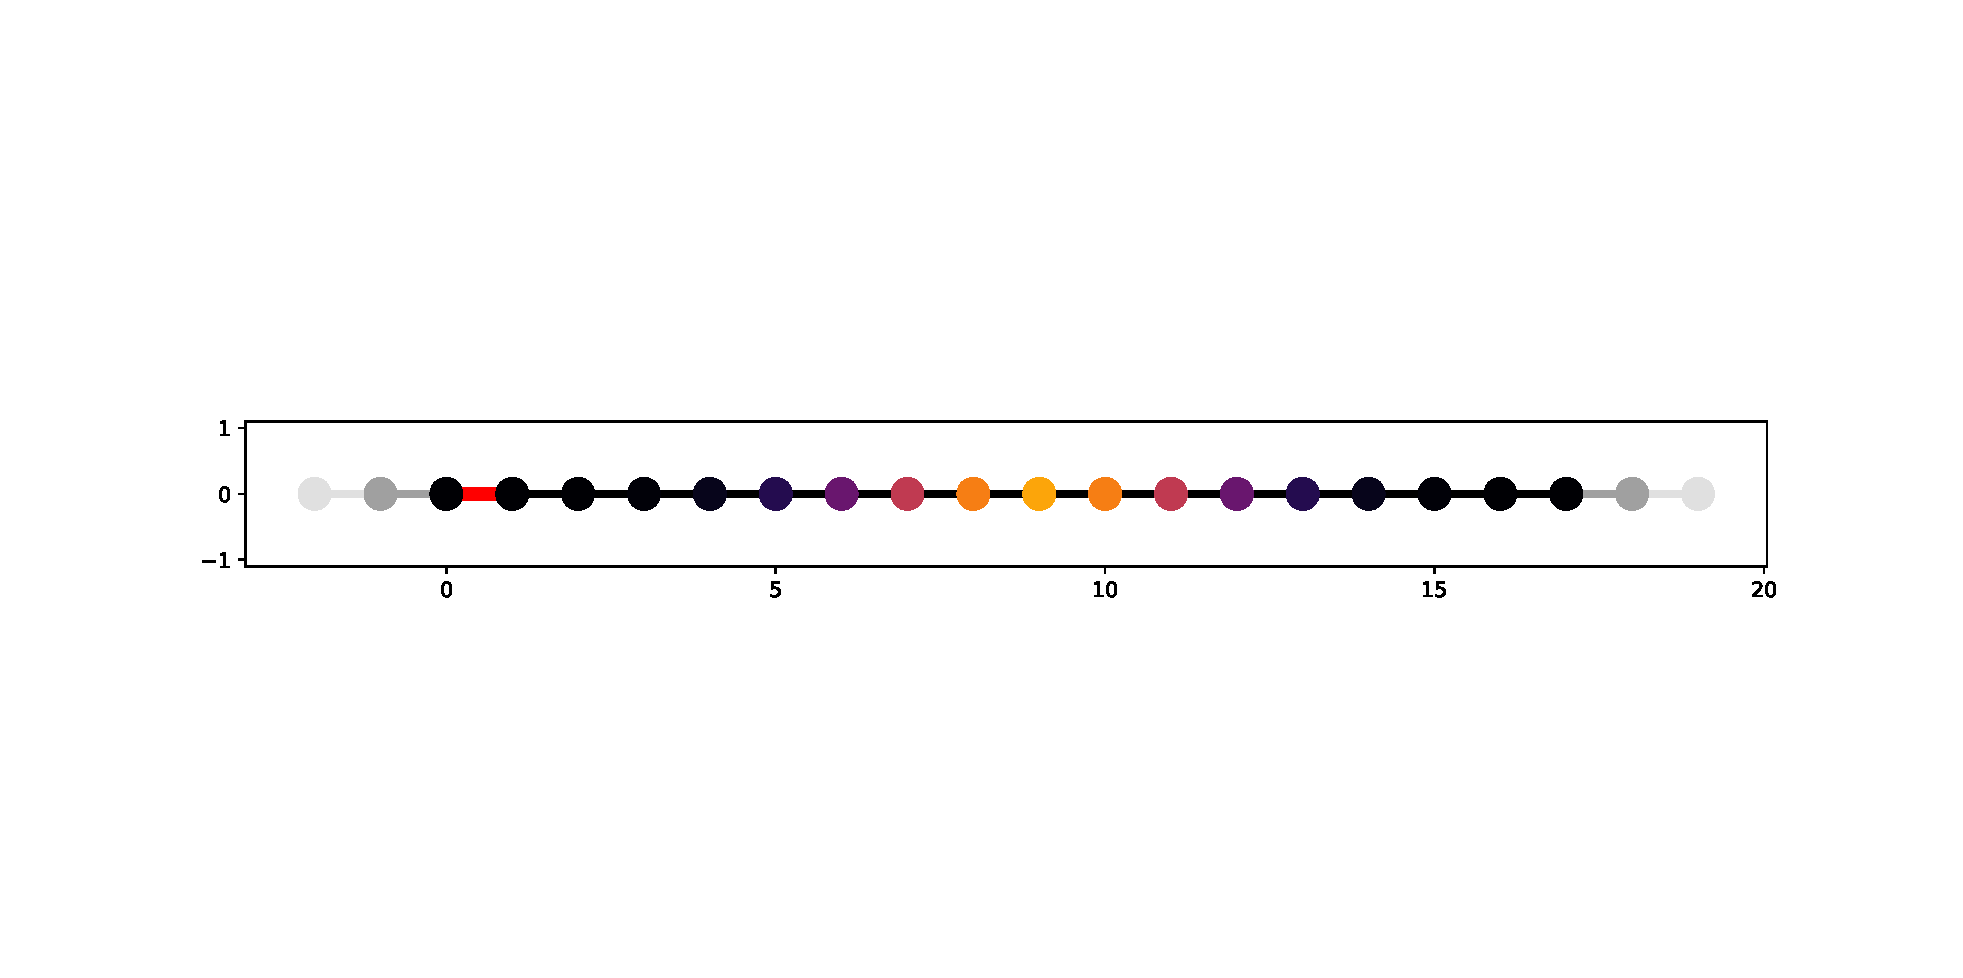
\includegraphics[width = 0.6\linewidth]{../figures/syst_color}
	\caption{A schematic of the system. The wire is connected to two semi-infinte leads. The site color reflects the QPC's voltage amplitude. The time-dependent hopping parameter is displayed in red. }
	\label{fig:systcolor}
\end{figure}
We consider a N sites one dimensional wire connected to two semi-infinite leads. We model the system by the following tight-binding Hamiltonian:
\begin{equation}
\textbf{H} = -\gamma \sum_{i}c^{\dagger}_i c_{i+1} + \sum_{i} w(t)\theta(-i) c^{\dagger}_i c_{i} + \sum_{i} V_{QPC}(i) c^{\dagger}_i c_{i}
\end{equation}
The scattering region will be indexed by $i \in [\![1,N]\!]$, whereas left (right) lead sites are indexed with $i \leq 0$
($i \geq N+1$). The voltage pulse is modeled by the second term, with $\theta(x)$ being the Heaviside function and $w(t)$:
\begin{equation}
w(t) = V_P e^{-2((t-t_0)/\tau)^2}
\end{equation}
$V_P$ being the amplitude, $\tau$ the width and $t_0$ the starting time of the perturbation. We introduced a Quantum Point Contact (QPC) which consists in a filtering potential barrier:
\begin{equation}
V_{QPC}(i) = V_0 e^{-((x-x_0)/\xi)^2}
\end{equation}
$V_0$ being the amplitude, $\xi$ the width and $x_0$ the position of the QPC.
The time-dependent peturbation can be absorbed by the gauge transforming leading to a redefinition of the hopping parameter the left lead where the pulse is applied and the scattering region:
\begin{equation}
\gamma \rightarrow \gamma e^{-i\phi(t)}
\end{equation}
with:
\begin{equation}
\phi(t) = \frac{e}{\hbar}\int_{-\infty}^{t} w(u)du
\end{equation}

\begin{figure}[h]
	\centering
	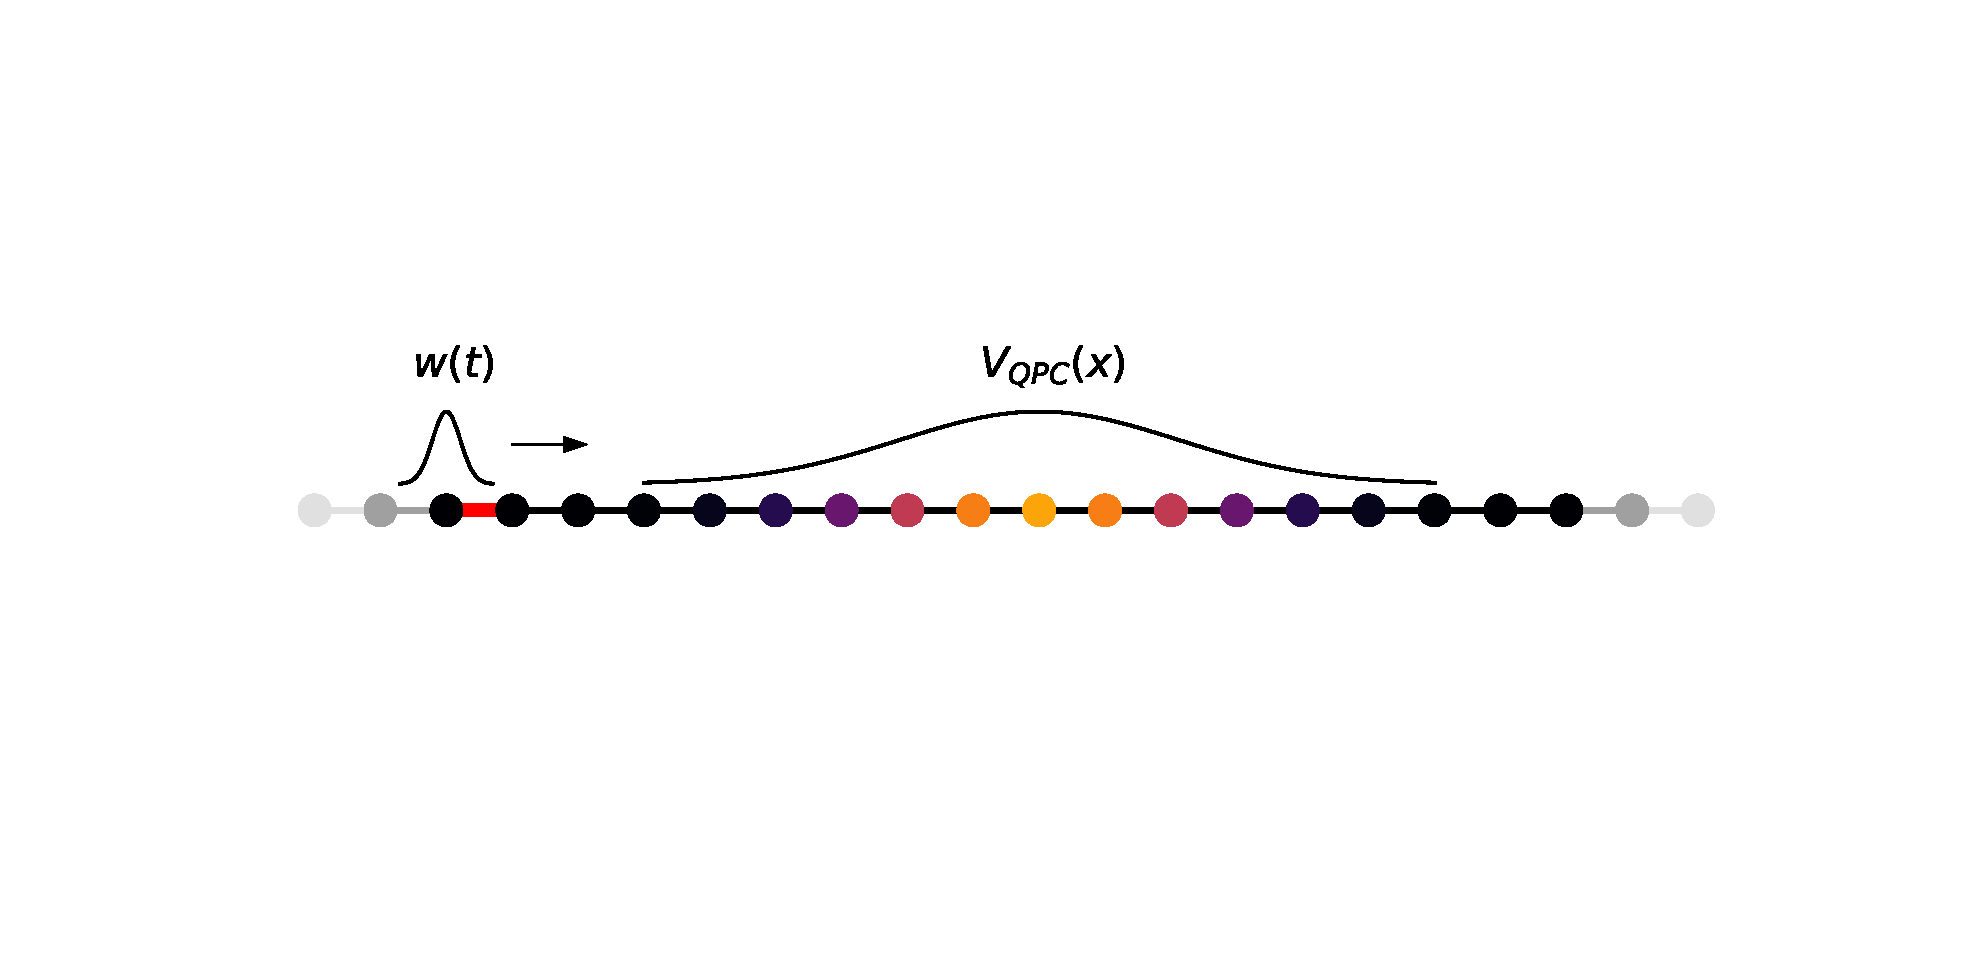
\includegraphics[trim=0cm 5cm 0cm 5cm, width = 0.9\linewidth]{../figures/syst_color_textv2}
	\caption{A schematic of the system. The wire is connected to two semi-infinte leads. The site color reflects the QPC's voltage amplitude. The time-dependent hopping parameter is displayed in red (here $L = 18$, $V_0 = 1$, $x_0 = L/2$, $\xi = 3$).}
	\label{fig:systcolor}
\end{figure}
\section{Simulation}
%Tkwant allows to evolve the states in time. The density is obtained by integrating over the energy of all onebody states:

\begin{equation}
n(i,t) = \int \frac{dE}{2\pi} f(E) |\psi(i,E)|^2
\end{equation}
\begin{figure}
	\centering
	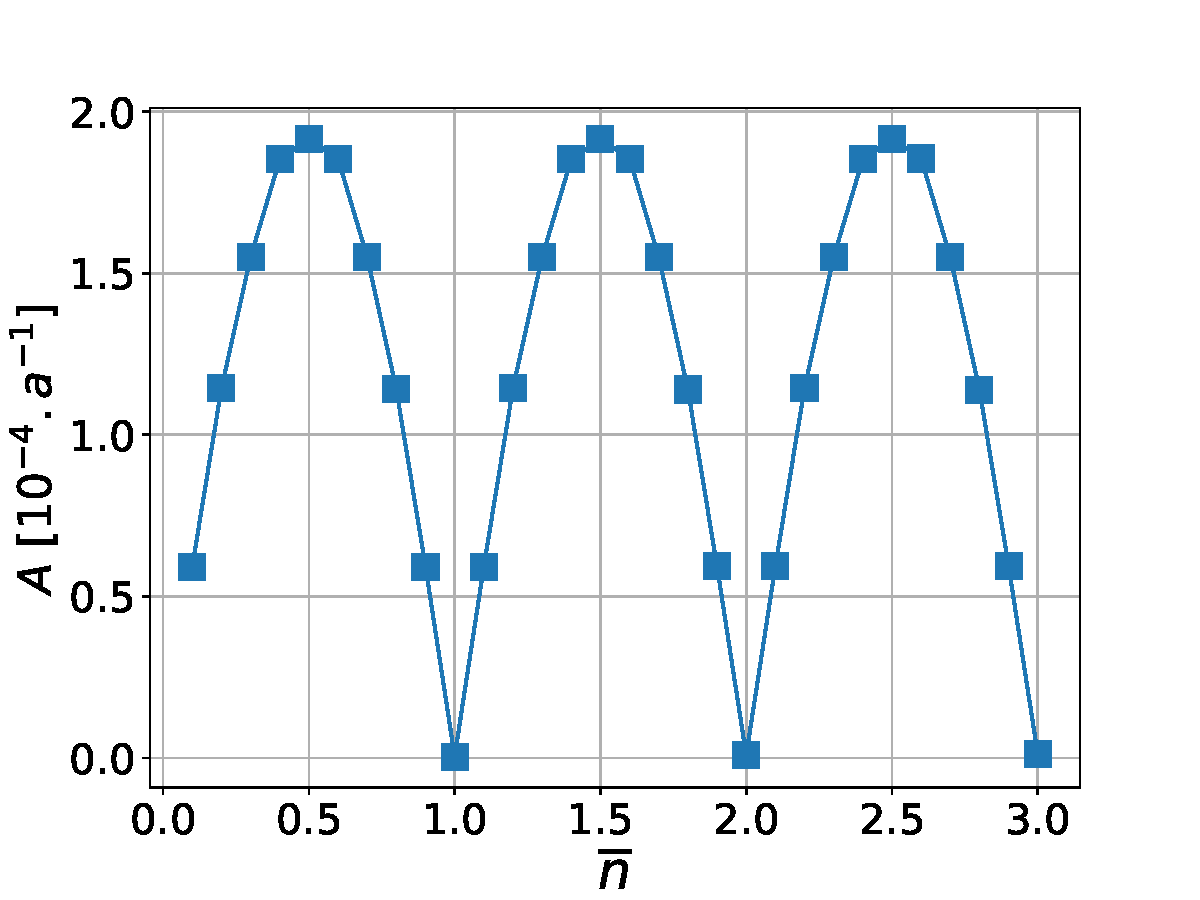
\includegraphics[width=0.7\linewidth]{../figures/A_vs_nbar_W1_L3000_V03_lx50_Ef21_u0_tau500}
	\caption{}
	\label{fig:avsnbarw1l3000v03lx50ef2}
\end{figure}

 Tkwant allows to evolve the states in time. The density is obtained by integrating over the energy of all onebody states:
 
 \begin{equation}
 n(i,t) = \int \frac{dE}{2\pi} f(E) |\psi(i,E)|^2
 \end{equation}
 
 We define the injected charge $\overline{n}$ as:
 \begin{equation}
 	\overline{n} = \int I(t)dt
 \end{equation}
 By using the Landauer-Büttiker formula $I = eV/h$, we obtain the following definition of $\overline{n}$:
 \begin{equation}
 	\overline{n} = \frac{eV_P\tau}{h}\sqrt{\frac{\pi}{2}}
 \end{equation}
 \begin{figure}
 	\centering
 	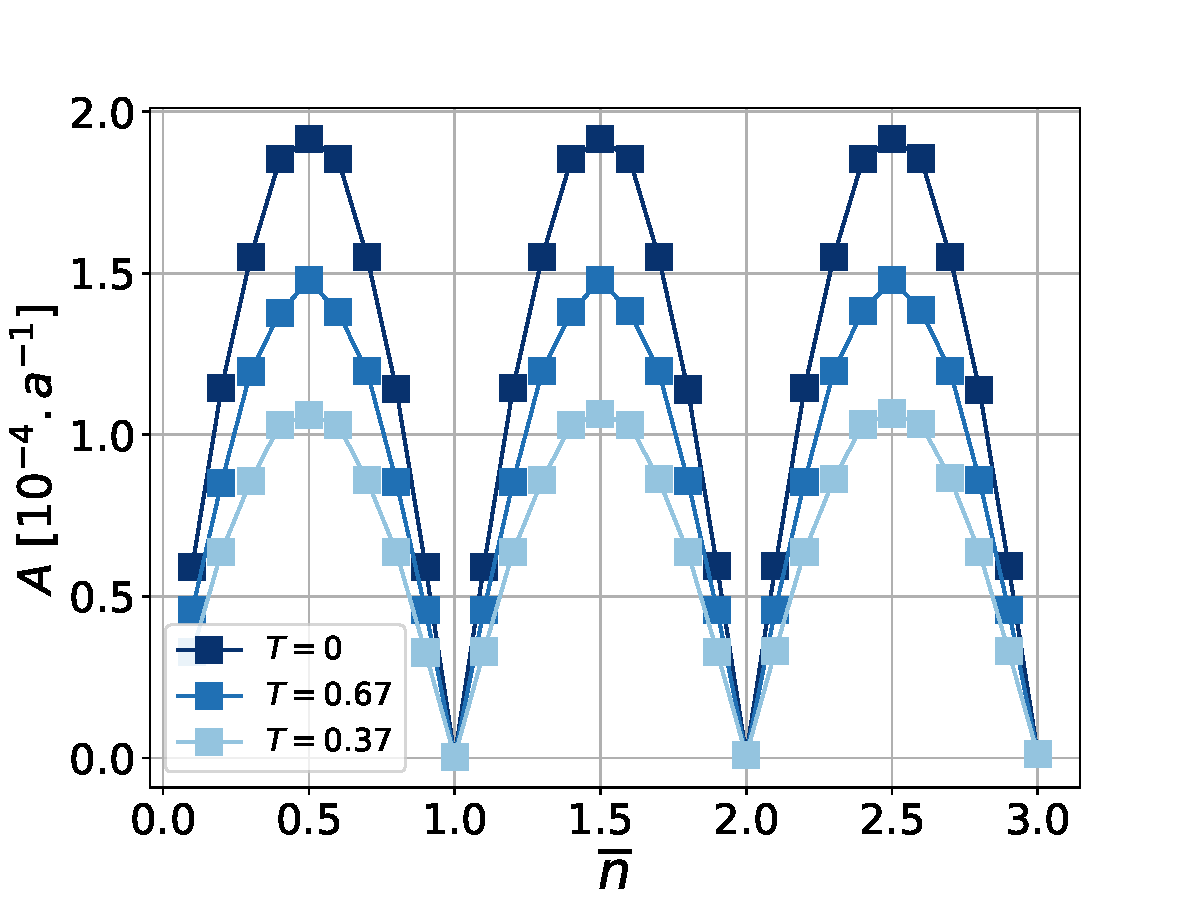
\includegraphics[width=0.7\linewidth]{../figures/A_vs_nbar_vs_transm}
 	\caption{The oscillation amplitude $A$ vs the injected charge $overline{n}$ for different values for transmission $T$. Here the parameters were: $W =1$, $L = 3000$, $\xi = 50$, $\tau = 500$, $t_0 = 1200$. For $T=0$, $V_0 =3$, $\xi = 50$, for $T=0.67$ ($T=0.37$), $V_0 =0.4$ ($V_0 = 0.24$) and $\xi = 1$.}
 	\label{fig:avsnbarw1l3000v03lx50ef2}
 \end{figure}
 
\section{Interferences}
For one-dimensional chain, the scattering states have the simple form:
\begin{equation}
	\psi(x,t) =  \frac{1}{\sqrt{v(k)}} e^{ikx - iEt}
\end{equation}

In our case, the QPC reflects the incoming states, and we obtain the following wavefunction:
\begin{equation}
\Psi(x,t) = \frac{1}{\sqrt{v(k)}} e^{ikx - iEt} + r\frac{1}{\sqrt{v(k)}} e^{-ikx - iEt}
\end{equation}

\begin{figure}[!h]
	\centering
	\subfloat[ ]{{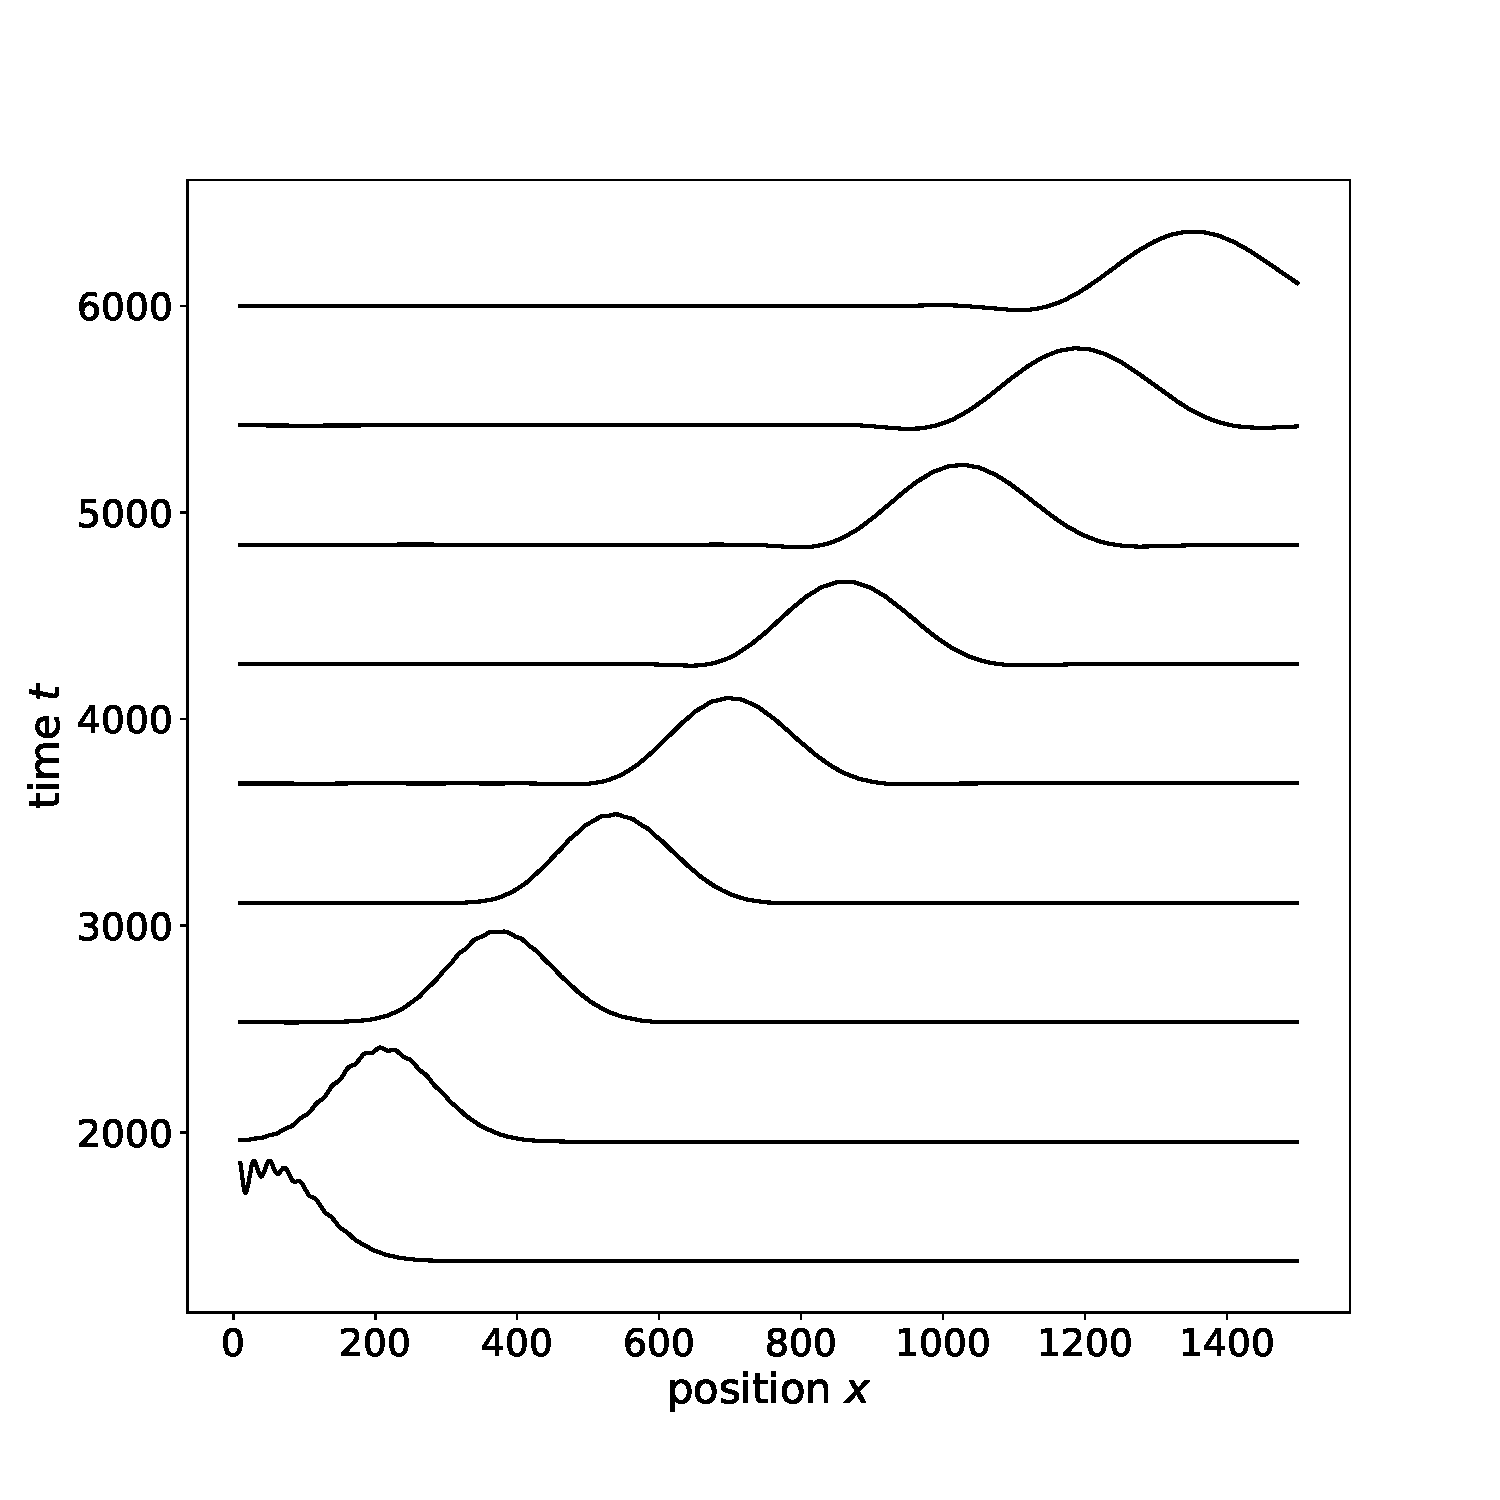
\includegraphics[width=0.4\linewidth]{../figures/density_off_202} }}%
	\qquad
	\subfloat[]{{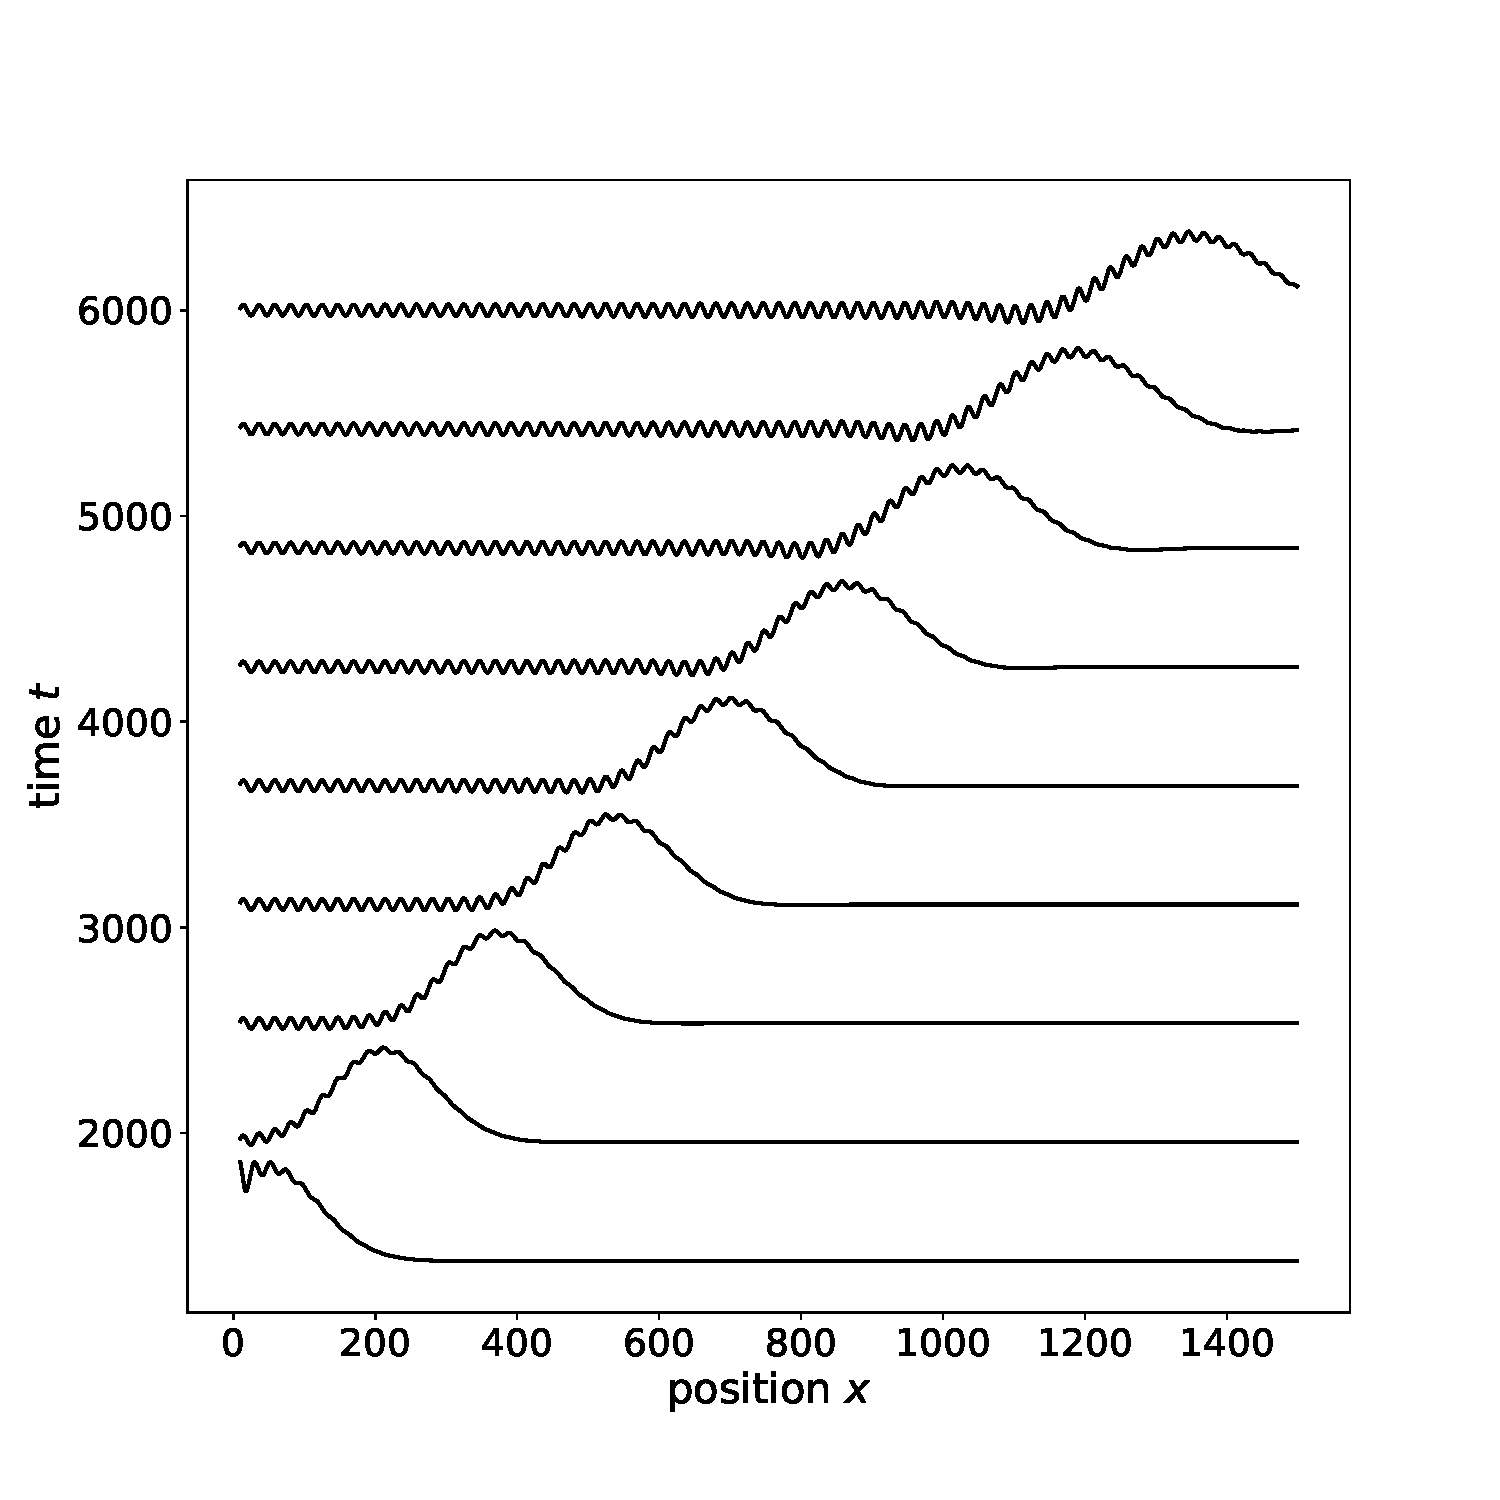
\includegraphics[width=0.4\linewidth]{../figures/density_on_202} }}%
	\caption{The charge density as a function of time $t$ and position $x$ (a) without (b) QPC. The parameters were $\overline{n} =0.01$, $\tau = 500$, $t_0 =1200$, (a) $V_0 = 0$ (b) $V_0 = 3$, $\xi = 50$, $E_F =2.02$.}
	
	\label{fig:density_comp}%
\end{figure}
\begin{figure}[!h]
	\centering
	\subfloat[ ]{{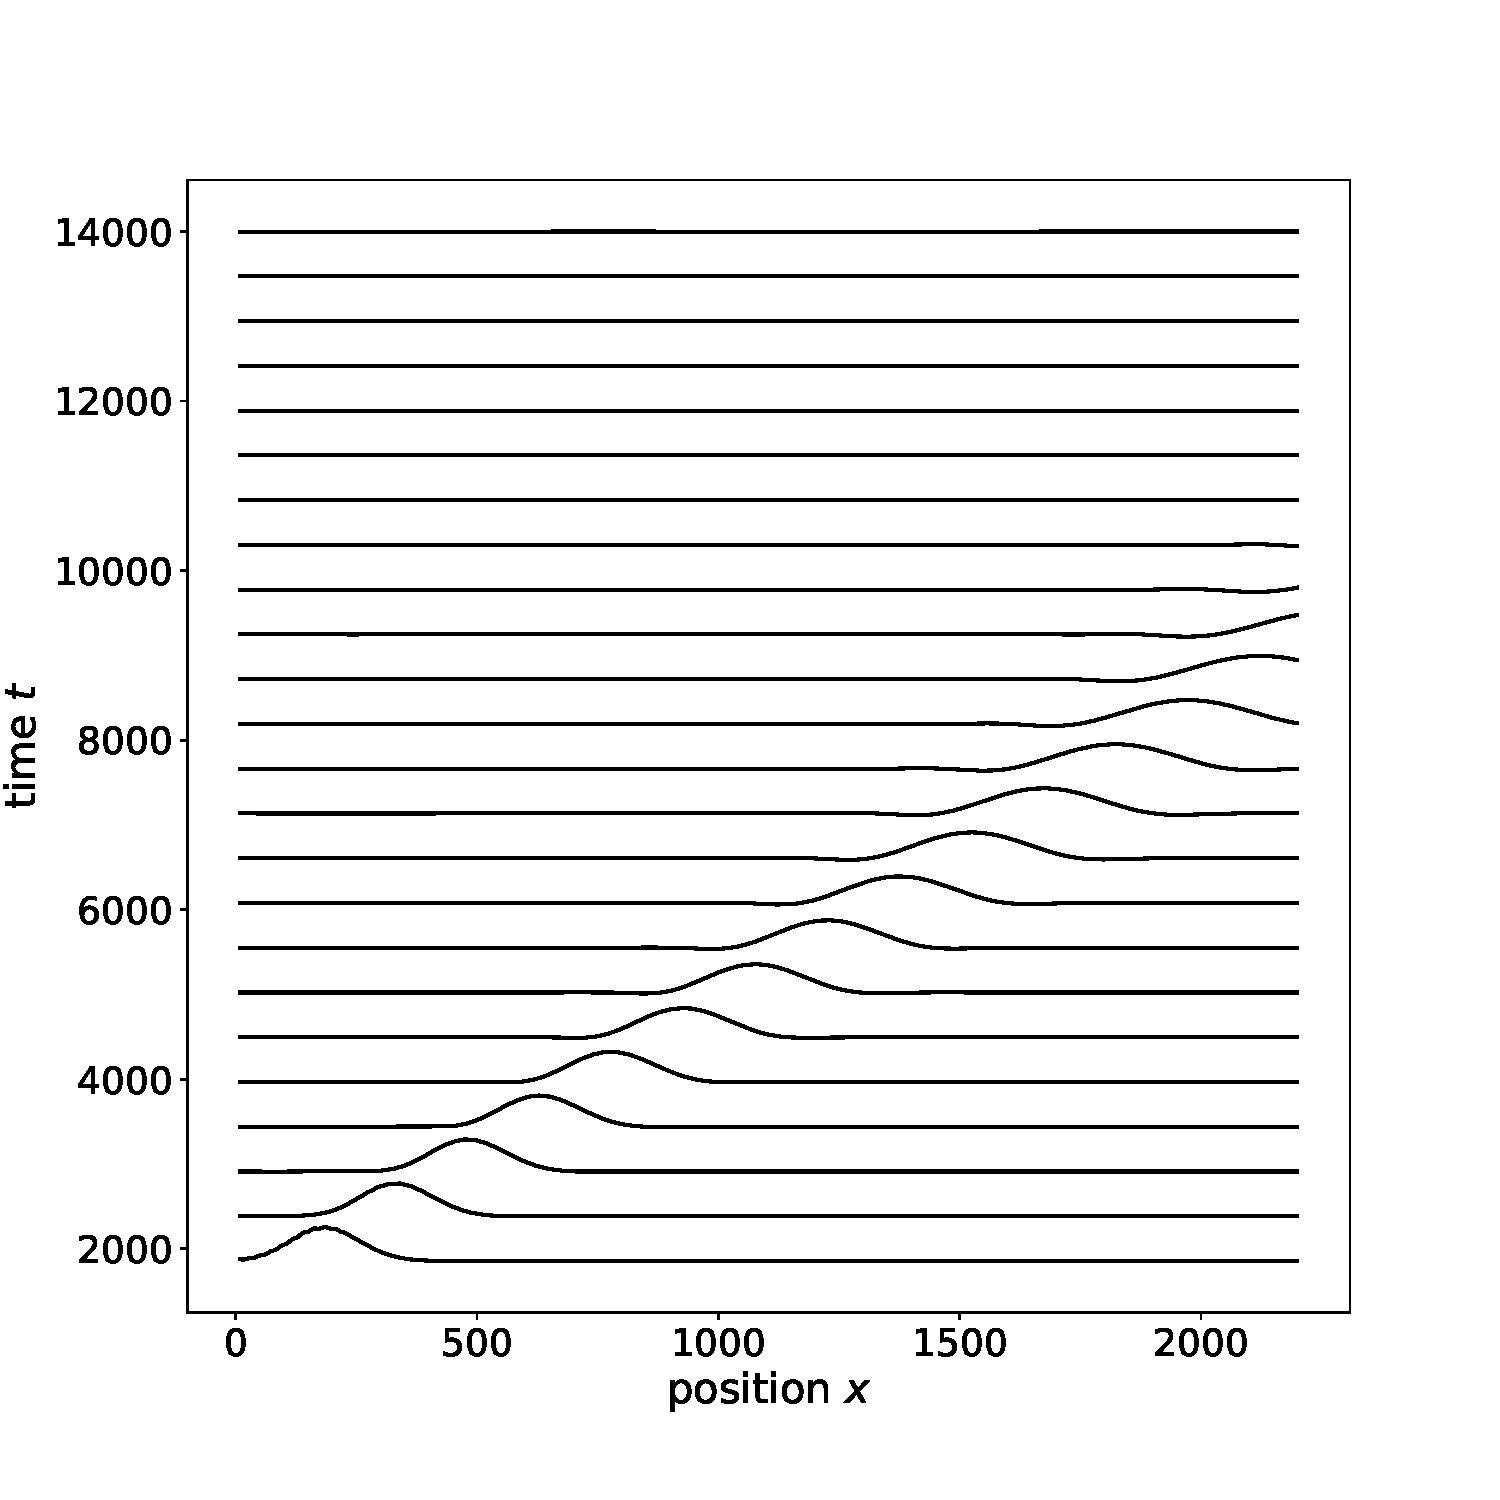
\includegraphics[width=0.4\linewidth]{../figures/density_off_202_reflection} }}%
	\qquad
	\subfloat[]{{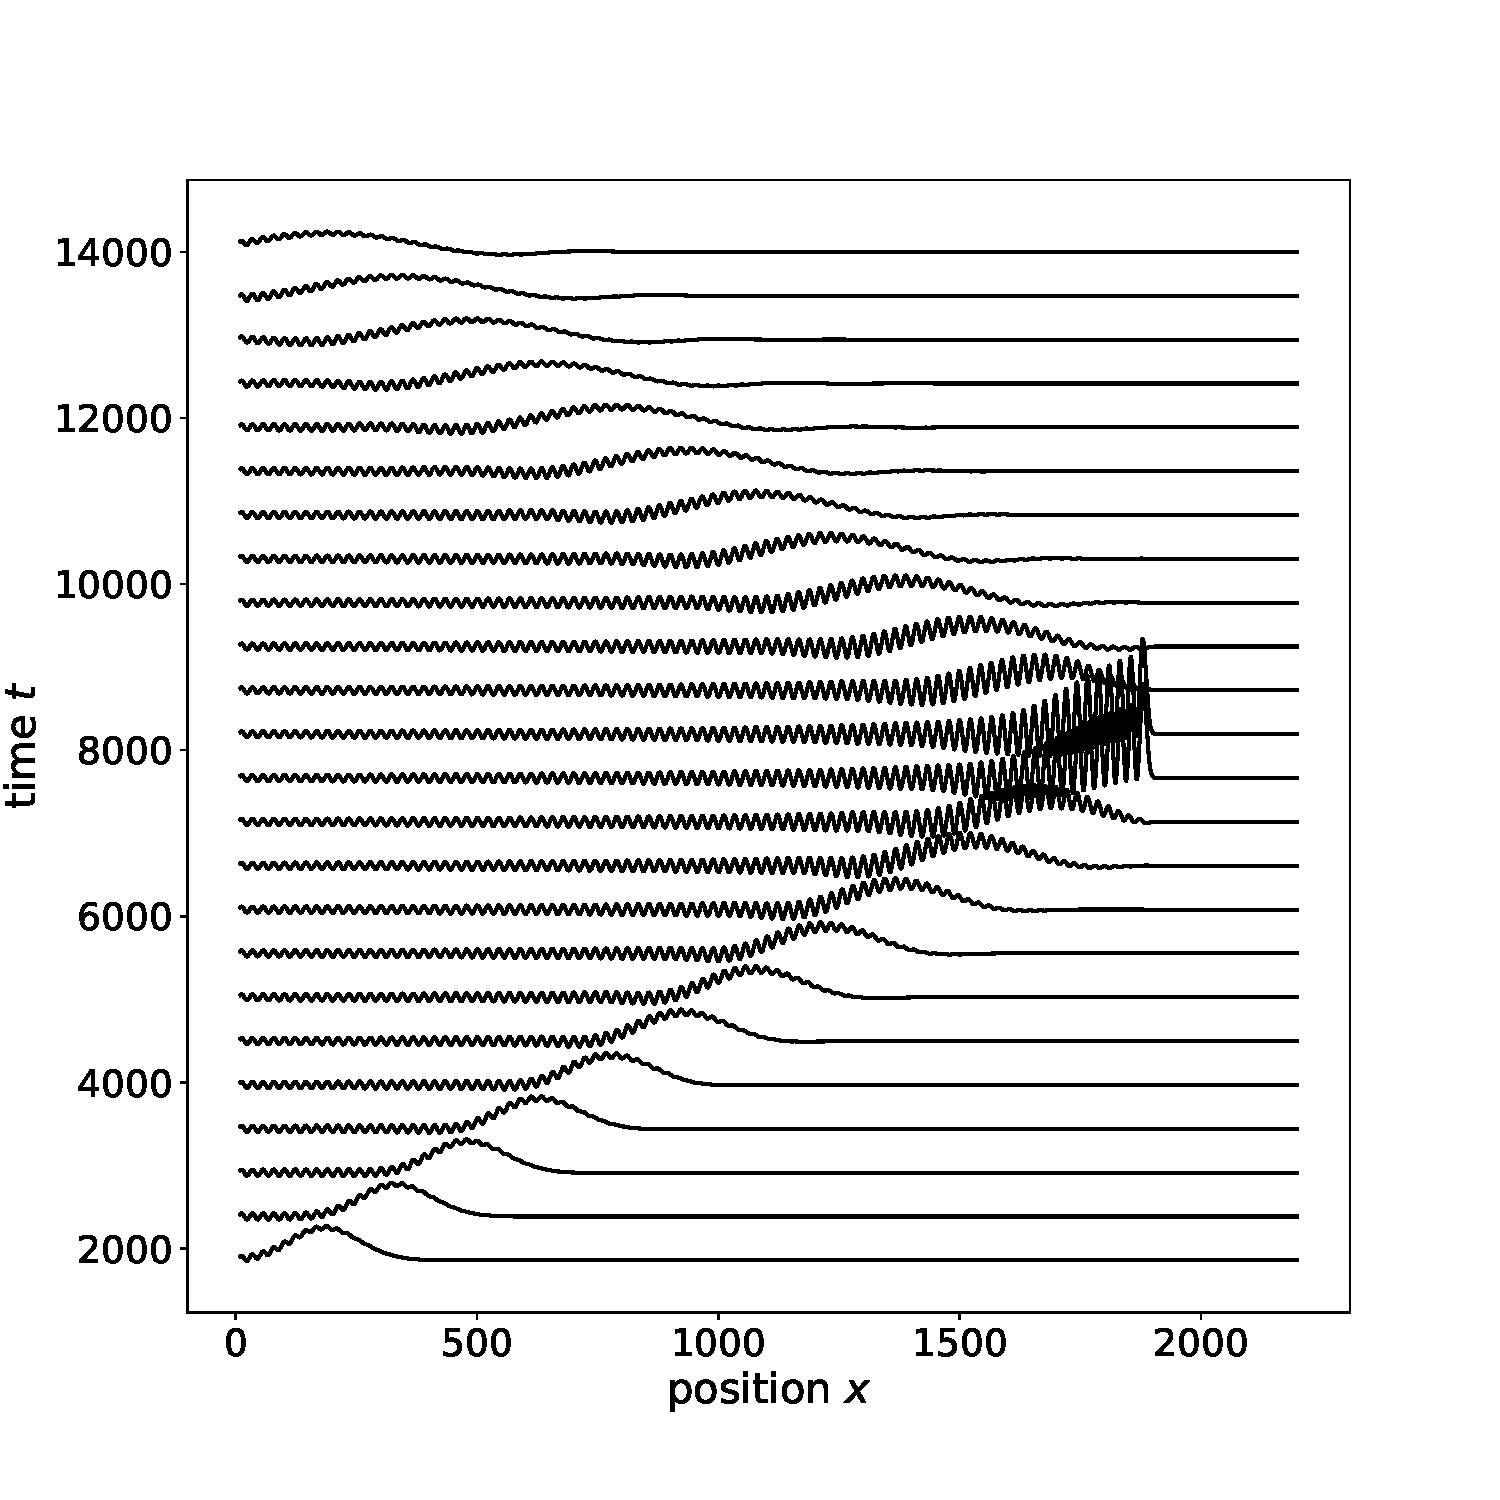
\includegraphics[width=0.4\linewidth]{../figures/density_on_202_reflection} }}%
	\caption{The charge density as a function of time $t$ and position $x$ (a) without (b) QPC. The parameters were $\overline{n} =0.01$, $\tau = 500$, $t_0 =1200$, (a) $V_0 = 0$ (b) $V_0 = 3$, $\xi = 50$, $E_F =2.02$.}
	
	\label{fig:density_comp_reflec}%
\end{figure}



This leads to destructive interferences. However, as the voltage pulse progagates, the incoming state phase shift dynamically:
\begin{equation}
\psi(x,t) =  \frac{1}{\sqrt{v(k)}} e^{ikx - iEt + i\phi(t)}
\end{equation}
which unveils the presence of interferences by changing the phase differences between the incoming and reflected states by $\phi(t\gg \tau) = 2\pi \overline{n}$.


\begin{figure}
	\centering
	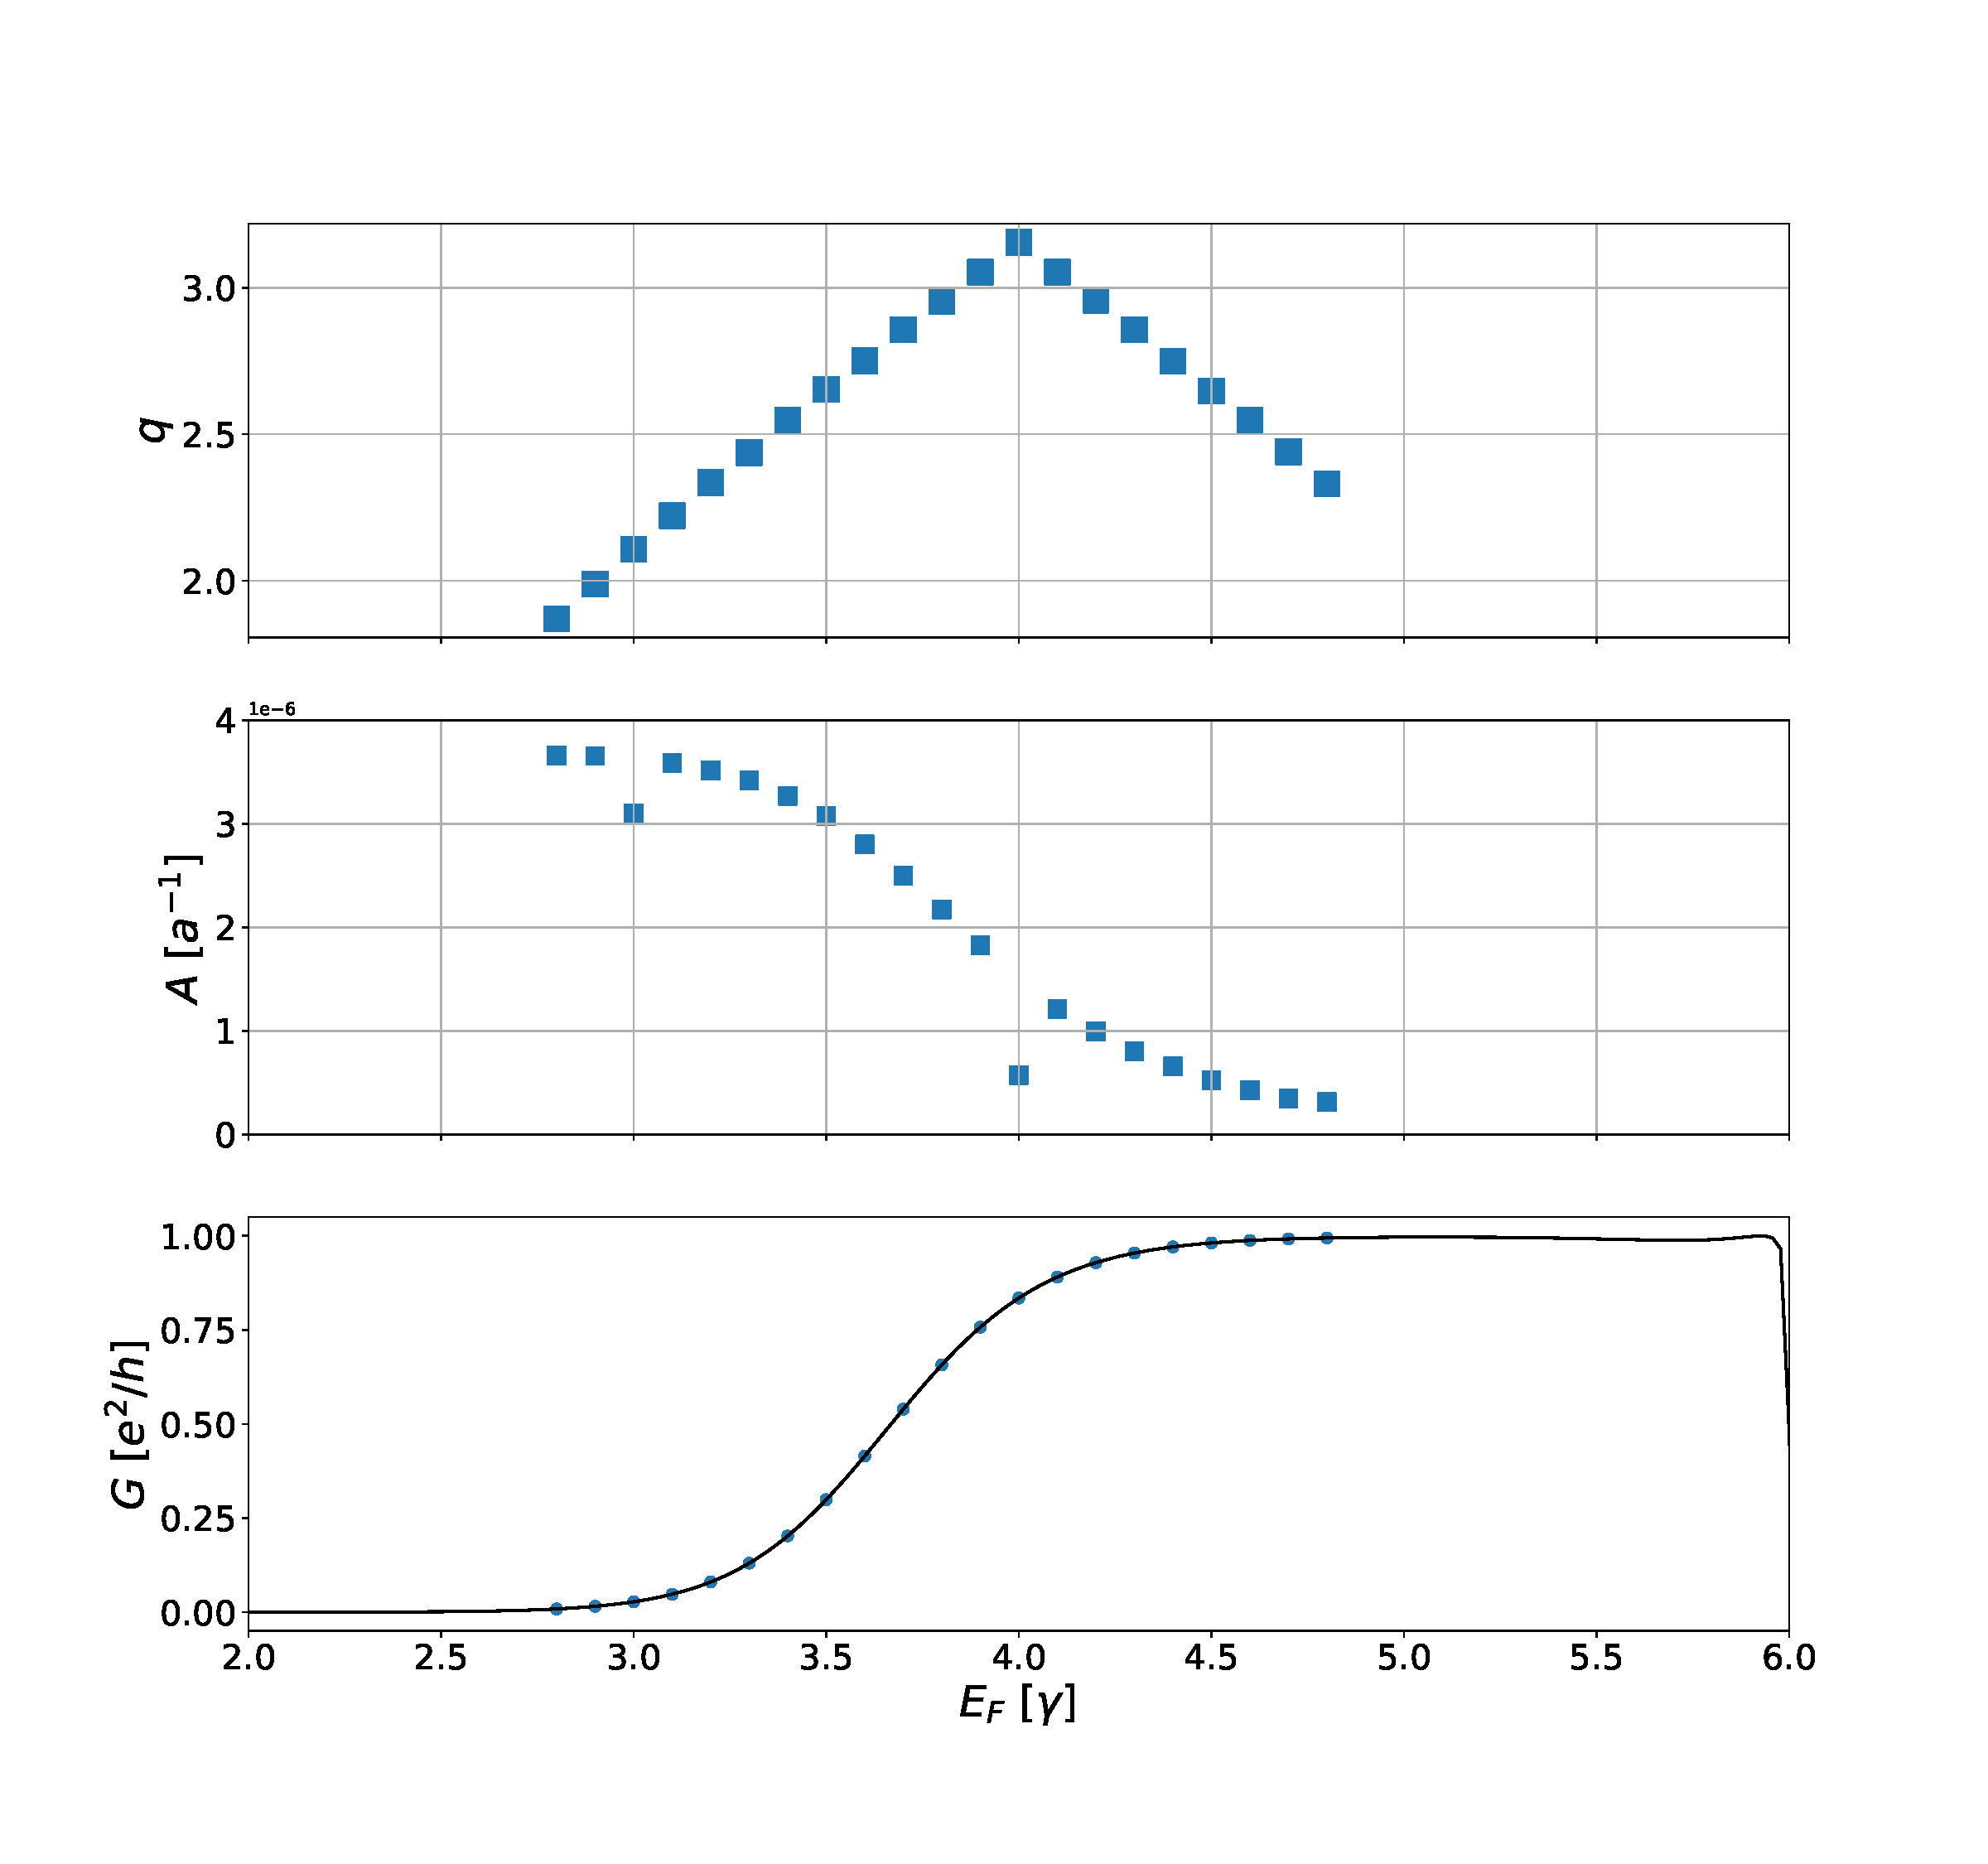
\includegraphics[width=0.7\linewidth]{../figures/G_AMP_Q}
	\caption{$L =4000$, $V_0 = 1.7$, $\xi = 2.1$}
	\label{fig:gampq}
\end{figure}


\begin{figure}
	\centering
	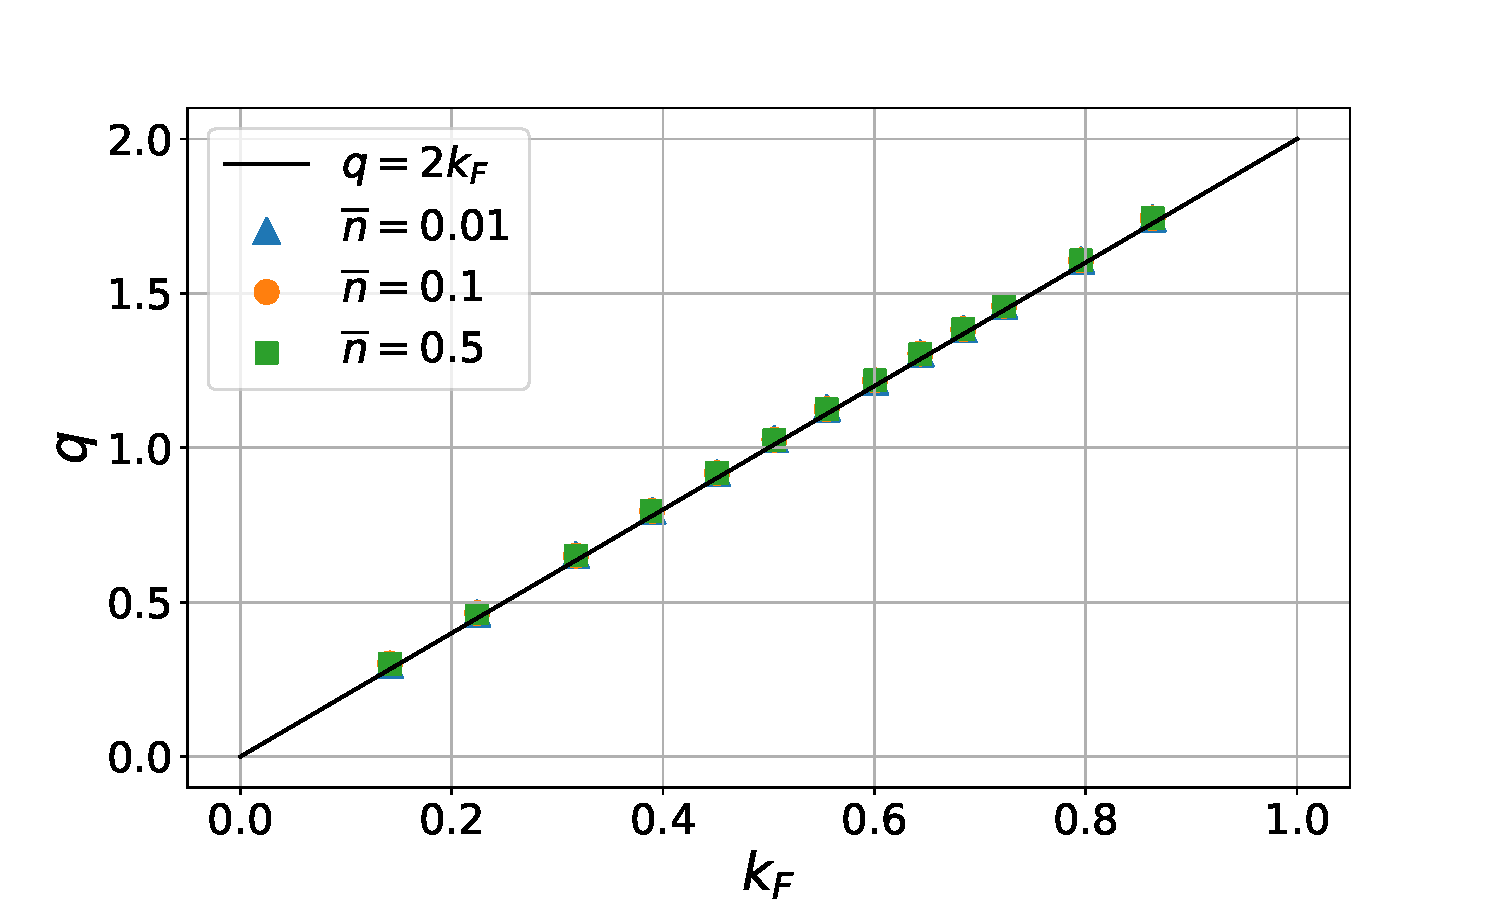
\includegraphics[width=0.7\linewidth]{../figures/q_vs_kf_differentnbar}
	\caption{The oscillation wavevector $q$ for different $k_F$ and $\overline{n}$ values. Here the parameters were: $L =3000$, $V_0 = 3$, $\xi = 50$, $\tau = 100$, $t_0 = 1200$.}
	\label{fig:qvskfdifferentnbar}
\end{figure}

\begin{figure}
	\centering
	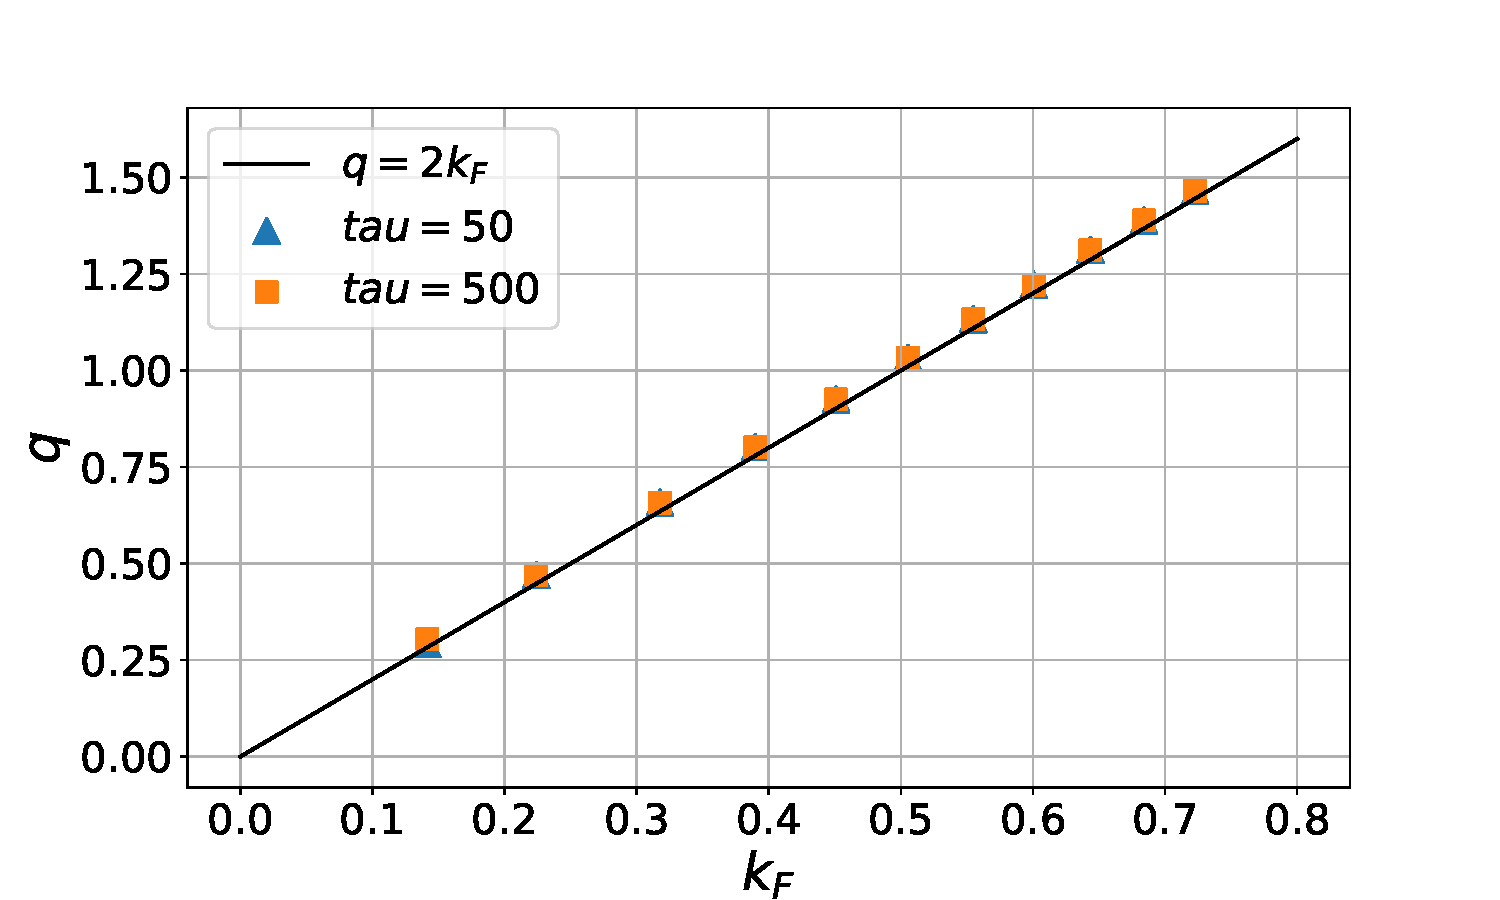
\includegraphics[width=0.7\linewidth]{../figures/q_vs_kf_differenttau}
	\caption{The oscillation wavevector $q$ for different $k_F$ and $\tau$ values. Here the parameters were: $L =3000$, $V_0 = 3$, $\xi = 50$, $\overline{n} = 0.01$, $t_0 = 1200$.}
	\label{fig:qvskfdifferenttau}
\end{figure}

\begin{figure}
	\centering
	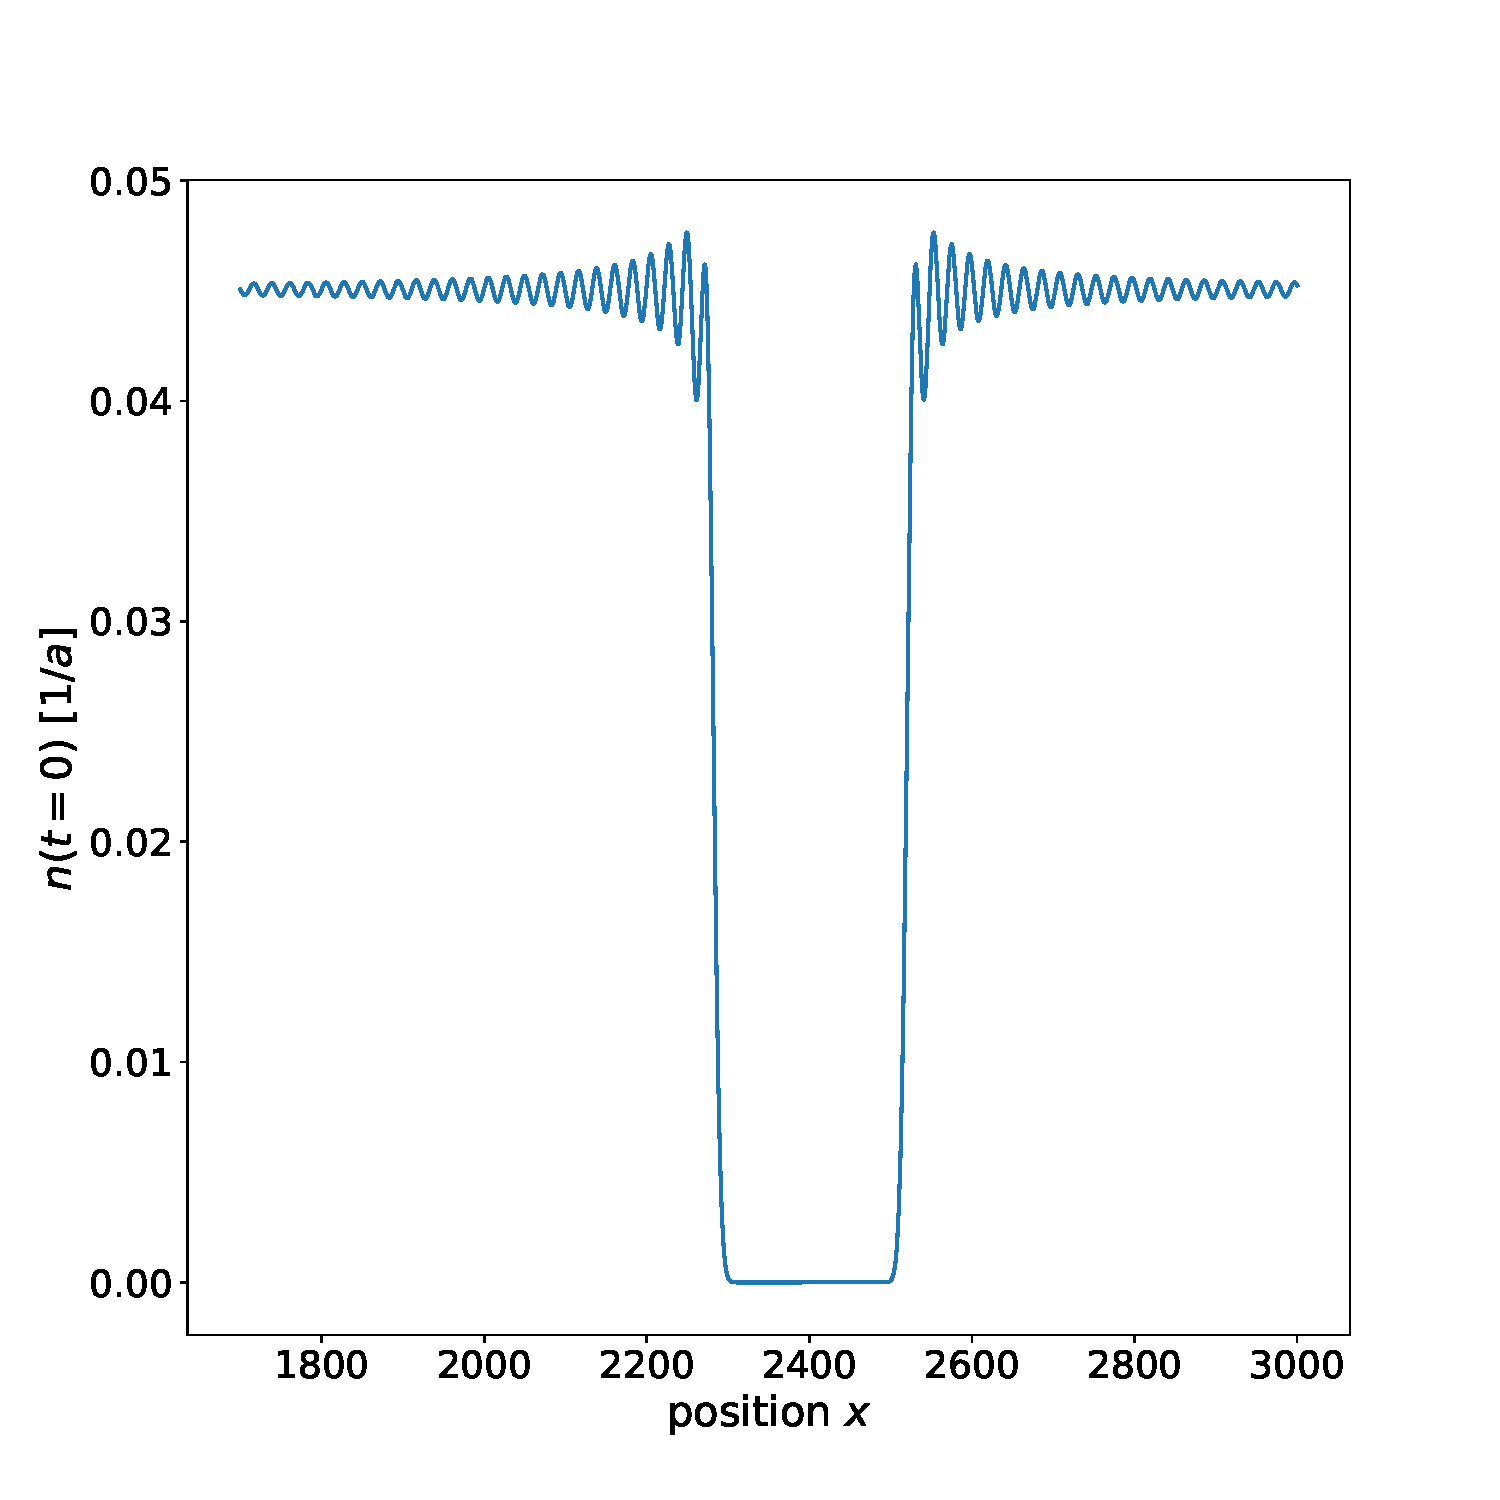
\includegraphics[width=0.7\linewidth]{../figures/oscillation_t0/plot_density_t0_Ef202}
	\caption{Density $n$ at t=0 for $\overline{n}$ = 0.01, $V_0$ =3, $E_F = 2.02$. We observe oscillation on both side of the QPC.}
	\label{fig:plotdensityt0ef202}
\end{figure}
\begin{figure}
	\centering
	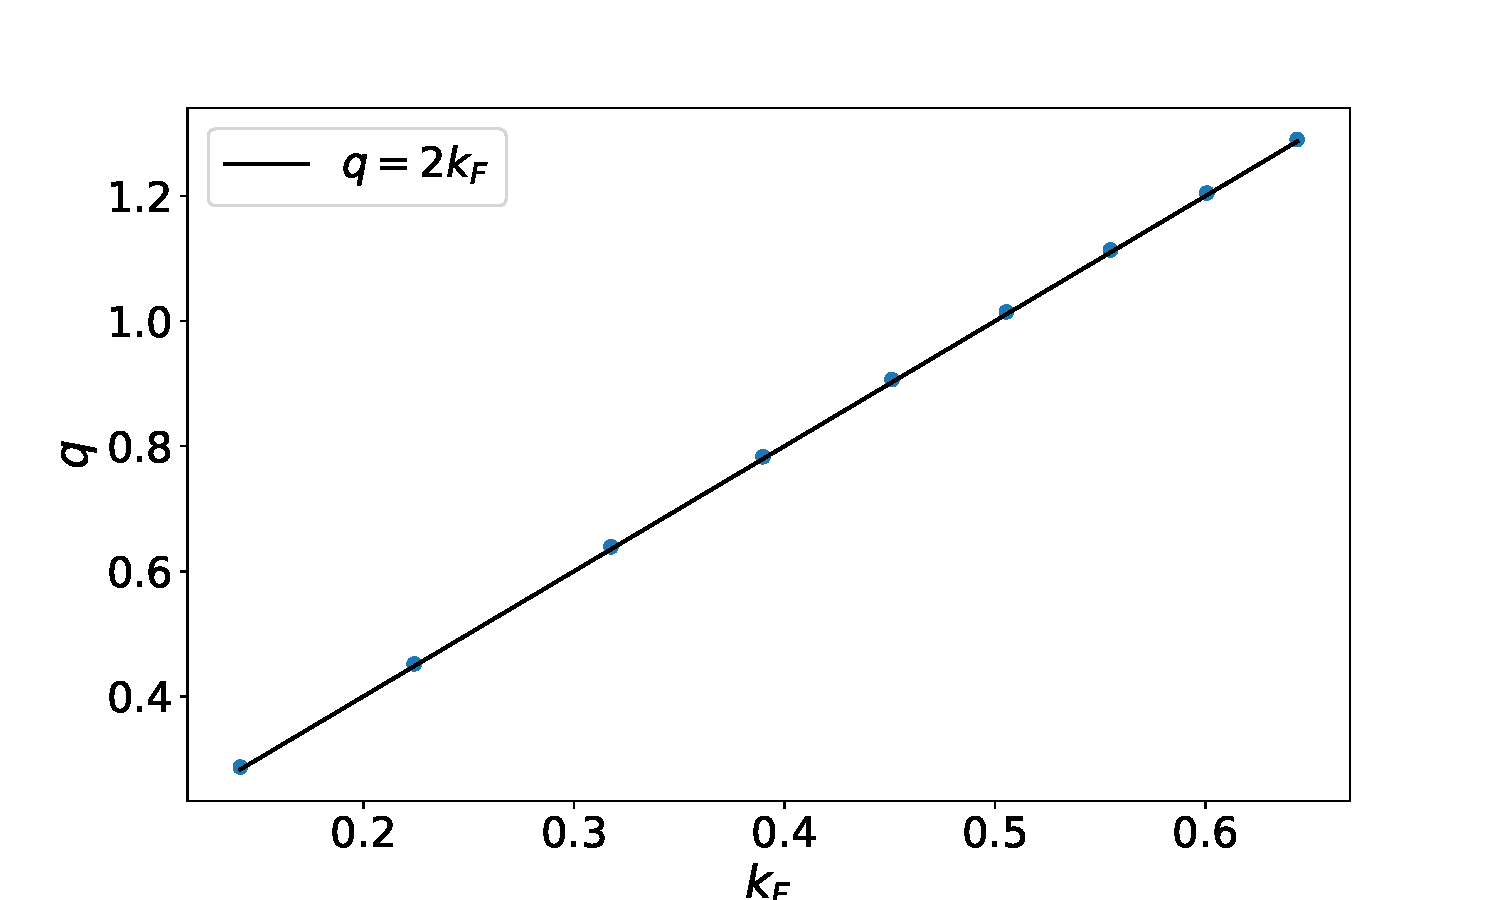
\includegraphics[width=0.7\linewidth]{../figures/oscillation_t0/q_vs_kf_at_t0}
	\caption{Oscillation wavevector $q$ of the oscillation at $t$=0 at differents $k_F$ values. There is a perfect match with the line $q = 2k_F$.}
	
	

	\label{fig:qvskfatt0}
\end{figure}

\begin{figure}
	\centering
	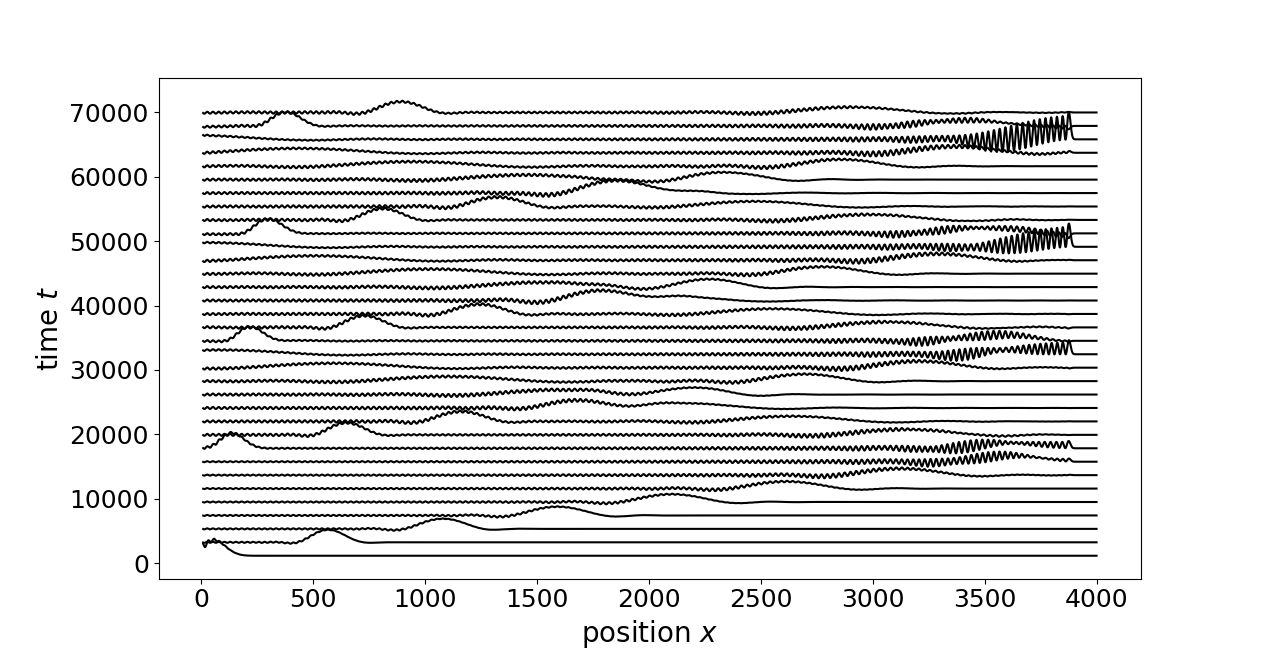
\includegraphics[width=0.7\linewidth]{../figures/1dwire_manypulse/plot_manypulse_L5000_V030_Ef2015_u00_n001}
	\caption{For $V_0$ = 3, $\overline{n}$ = 0.01, $E_F$ = 2.015, we send a new pulse everytime a pulse reaches the QPC. In some region, the oscillation seems to be quasi-stationnary.  }	\label{fig:plotmanypulsel5000v03}
\end{figure}



\bibliography{basename of .bib file}

\end{document}
%
% ****** End of file apstemplate.tex ******
% If in two-column mode, this environment will change to single-column
% format so that long equations can be displayed. Use
% sparingly.
%\begin{widetext}
% put long equation here
%\end{widetext}

% figures should be put into the text as floats.
% Use the graphics or graphicx packages (distributed with LaTeX2e)
% and the \includegraphics macro defined in those packages.
% See the LaTeX Graphics Companion by Michel Goosens, Sebastian Rahtz,
% and Frank Mittelbach for instance.
%
% Here is an example of the general form of a figure:
% Fill in the caption in the braces of the \caption{} command. Put the label
% that you will use with \ref{} command in the braces of the \label{} command.
% Use the figure* environment if the figure should span across the
% entire page. There is no need to do explicit centering.

% \begin{figure}
% \includegraphics{}%
% \caption{\label{}}
% \end{figure}

% Surround figure environment with turnpage environment for landscape
% figure
% \begin{turnpage}
% \begin{figure}
% \includegraphics{}%
% \caption{\label{}}
% \end{figure}
% \end{turnpage}

% tables should appear as floats within the text
%
% Here is an example of the general form of a table:
% Fill in the caption in the braces of the \caption{} command. Put the label
% that you will use with \ref{} command in the braces of the \label{} command.
% Insert the column specifiers (l, r, c, d, etc.) in the empty braces of the
% \begin{tabular}{} command.
% The ruledtabular enviroment adds doubled rules to table and sets a
% reasonable default table settings.
% Use the table* environment to get a full-width table in two-column
% Add \usepackage{longtable} and the longtable (or longtable*}
% environment for nicely formatted long tables. Or use the the [H]
% placement option to break a long table (with less control than 
% in longtable).
% \begin{table}%[H] add [H] placement to break table across pages
% \caption{\label{}}
% \begin{ruledtabular}
% \begin{tabular}{}
% Lines of table here ending with \\
% \end{tabular}
% \end{ruledtabular}
% \end{table}

% Surround table environment with turnpage environment for landscape
% table
% \begin{turnpage}
% \begin{table}
% \caption{\label{}}
% \begin{ruledtabular}
% \begin{tabular}{}
% \end{tabular}
% \end{ruledtabular}
% \end{table}
% \end{turnpage}

% Specify following sections are appendices. Use \appendix* if there
% only one appendix.
%\appendix
%\section{}

% If you have acknowledgments, this puts in the proper section head.
%\begin{acknowledgments}
% put your acknowledgments here.
%\end{acknowledgments}

% Create the reference section using BibTeX: